\documentclass[12pt]{article}

%
%Margin - 1 inch on all sides
%
\usepackage[letterpaper]{geometry}
\geometry{top=1.0in, bottom=1.0in, left=1.0in, right=1.0in}

%
%Doublespacing
%
\usepackage{setspace}
\doublespacing

% 
%Babel package for multiple language typesetting
%
%\usepackage[english,spanish]{babel}
%\usepackage[T1]{fontenc}
%\usepackage[latin1]{inputenc}

%
%Setting the font
%G
\usepackage{times}
\usepackage{graphicx}

\renewcommand{\thesection}{\arabic{section}.}

%
%Works cited environment
%(to start, use \begin{workscited...}, each entry preceded by \bibent)
% - from Ryan Alcock's MLA style file
%
\newcommand{\bibent}{\noindent \hangindent 40pt}
\newenvironment{workscited}{\newpage \begin{center} Works Cited \end{center}}{\newpage }

\newcommand{\mc}{M\'airt\'in}
\newcommand{\mcs}{M\'airt\'in }

%
%Begin document
%
\begin{document}
\begin{flushleft}

%%%%First page name, class, etc
Michael Gilliland \\
Dr. Lynda Szabo \\
Humanities 203 \\
\today \\
Words: 1395 \\

%%%%Title
\begin{center}
{\large The New Style of Christian Thought}
\end{center}

%%%%Changes paragraph indentation to 0.5in
\setlength{\parindent}{0.5in} 

%START%

\section{Introduction}

This life is a journey. In it we encounter not only obstacles, triumphs and
failures but also multitudes of opinions, views and philosophies. Our 
perception of these philosophies, through rejection or acceptance can even 
entail successful survival and -- as many Christians would argue -- 
\emph{correct} survival. The ``Allegory of the Theologians'' is a mechanism
for analyzing content from four different perspectives: literal, allegorical,
moral and anagogical. The literal perspective is concerned with the details of
what actually happened, it is narrative in nature. The allegorical perspective
is used to evaluate events and art not for exactly what occurrences they contain but for
what said occurrences symbolize. Proper use of the moral perspective
entails understanding events and artistic forms as they pertain to our choices in life;
it helps us know how we should live our lives. Lastly, the anagogical perspective is
concerned with studying depictive forms for the understanding of our destiny,
to discover where we end up. I claim that Medieval Christian architecture, and
literature (such as \emph{Dante's Inferno}) illustrate that modern Christians
hold significantly different views on Christianity than the Medieval
Christians held.

\section{Chartres Cathedral}

\begin{center}
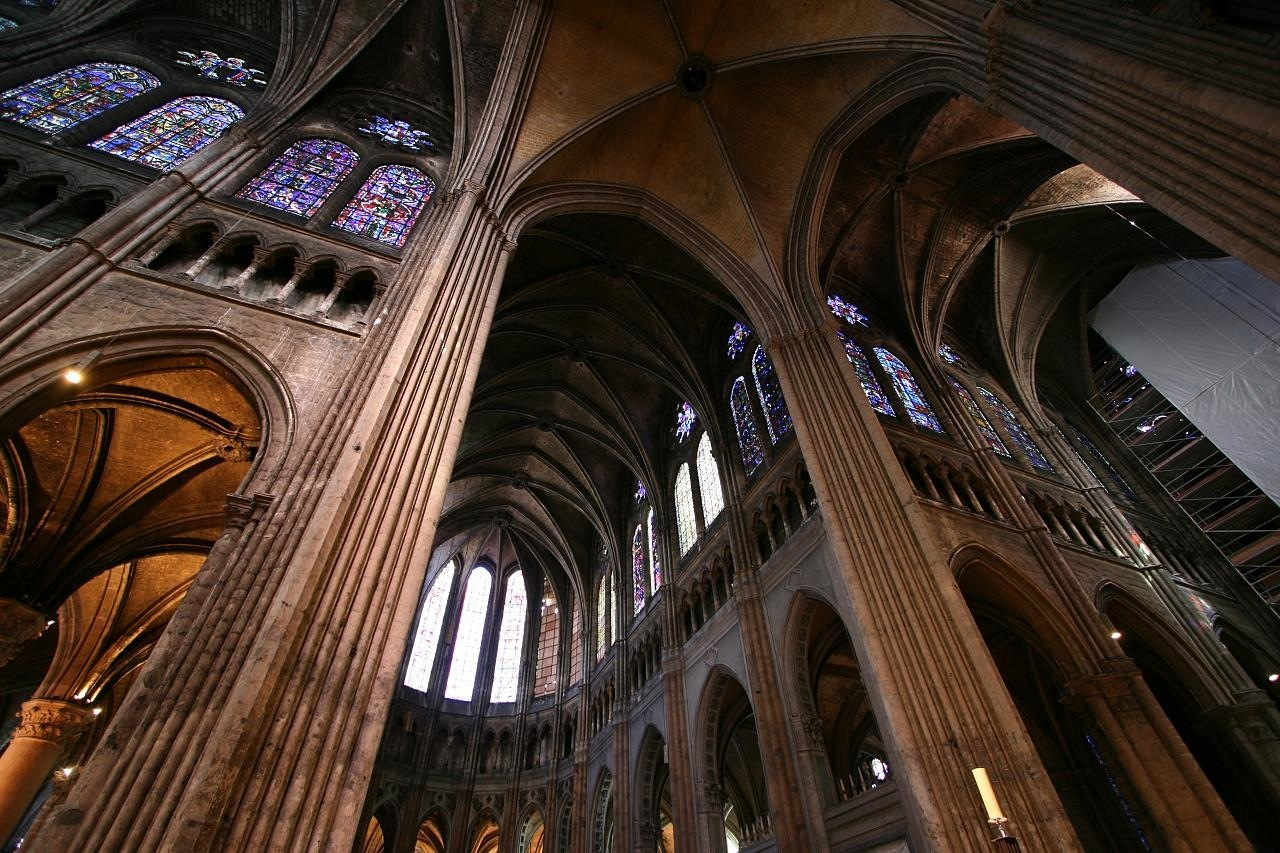
\includegraphics[scale=0.3]{InteriorAtTheCrossing.png} \\
{\bf Figure 1: Interior, at the Crossing}
\end{center}

The above image of the interior ceiling of Chartres Cathedral is a prime
example of this difference in thought. In a literal
view we see a huge structure with many archways. We see a couple of 
lights, however, most of the lighting comes from the many windows
(most of which are stained glass, few of which are not). In the literal
sense we can reasonable conclude that this cathedral is architectural
marvel that surely costed a fortune. This literal interpretation 
reflects into the allegorical interpretation. The light coming into the
church is symbolic of Christ as the ``light of the world'' and also of
church-goers as being ``children of light'' (Cite...). The size and the
many arches seem to be declaring the glory of the church.

The third mechanism, the moral interpretation that the cathedral provides
is one of distance. The cathedral's huge size coupled with the hight of
the ceiling seems to imply a distant, almost fearful relationship with God.
It implies that Christians are lowly and ought to have a great fear of a
great God. Even the high placement of the stain glass windows, depicting
Bible stories, seems to emphasize the distance between God (along with things of
God) and man. The anagogical perspective is, in may respects, derivative
of the other three interpretations (especially the moral). The supreme distance
reminds us that heaven is not close to us, it is not of this world. The beauty
and complexity of the cathedral inspire reverence implying that heaven will
be a large, sanctuary-like haven for those who have adequate reverence and fear
of the Lord. Overall, Chartres Cathedral presents the Medieval church's
high view of heaven as a far off and beautiful place. The cathedral serves
as an architectural modelling of the Medievals' view of heaven. To every coin
there is a flip-side. To present their view of hell, I will next examine the
5th Canto of \emph{Dante's Inferno} and the themes that proceed from therein and
are present throughout the rest of the book.

\section{\emph{Dante's Inferno}}

By literal analysis, the reader is show Dante and Virgil entering the second
circle of hell (it is divided up into rings). They then see a large, 
specie-less creature named Minos, having a long tail. Minos wraps its tail
around sinners entering hell, encircling them a number of times specifying
the number of the circle of hell in which they will reside perpetually (Dante 37). The
canto continues on, pointing out individual sinners who are entering, however,
I will focus on the former details and what they entail throughout the story.
From the allegorical perspective, this canto has implications throughout the rest of
the book. Allegorically, the very fact that there is assignment implies that
there are different levels of sin (i.e. some sins are worse than others).
The different circles of hell (and the different punishments) imply that
hell has no uniform method of punishing sinners, and the different sins
in life merit different punishments in the afterlife.

Using the moral perspective from ``Allegory of the Theologians,'' we see
that the process of the allocation in hell for different sins provides
a clear model on how Medieval Christians should live their lives. By
Dante's normative, Christian's ought to live their lives in repentance
walking the straight path and that we ought not, as he says through 
Odysseus in canto XXVI, ``live as a mere brute does, [b]ut for the 
pursuit of knowledge and the good'' (Dante 223) His assignment of perpetrators to the center
circle (where the punishment is the worst) shows Medieval Christians
that fraud is the worst sin they can commit and that some sins can be
categorized into different magnitudes of wrongdoing. As stated earlier,
where Chartres Cathedral presents a model of heaven after earth, 
\emph{Dante's Inferno} paints a picture of hell. Anagogically, and very clearly, Dante is
saying that people, even those claiming to be Christians, who live 
non-repentant lives will suffer perpetually and physically in hell. The
physical pain is the main component he stresses, as the sins and punishments
grow increasingly "worse" and he explores the deeper recesses of hell. Also,
Dante presents a singular, one-to-one nature of punishments to crimes.

\section{Conclusion}

The Medievals' line of thinking seems to be very discrete and physical in
nature. For example, in Chartres Cathedral, the emphasis of the church is in
the building itself, the magnificence and glory of the structure. In 
\emph{Dante's Inferno}, hell is described as categorical sinners' pidgin-holes,
the purpose of which is physical torment for eternity. Dante makes clear
distinctions regarding the ``magnitude of sin,'' and his tailored symbolic
retributions. As stated earlier, I believe that modern Christian views digress
from the Medievals' views of the Christian life and afterlife. Where Chartres
Cathedral symbolizes a distance between God and the individual, modern
Christians speak of a \emph{personal} relationship with God (through Christ),
and they call themselves ``friends of God.'' Where the cathedral in itself
is the emphasis of the cathedral, modern Christians believe that the people
are the church, and that the building is secondary. Regarding Dante's view
of life and hell, modern Christians will contest that ``a sin is a sin'' and
will state that the only true punishment in hell is eternal separation from 
Christ.

Although I believe that the Christians of the present day would disagree with
many of the themes of Chartres Cathedral and \emph{Dante's Inferno}, I also
believe they would find some virtue and worth in their methods of making
sense of the world. Though extravagant and non-simplistic, the cathedral
with the intend of being a tribute to Christianity and a place of worship.
These attributes are irrefutable by modern Christians. \emph{Dante's Inferno}
is, in essence, an anagogical book which seems to almost use a scare-tactic
to illustrate to Medieval Christians what will happen to them if they fail
to live as they \emph{should}. Contrarily, modern Christians hold relationships
with Christ above acts, and separation from Christ as being worst than physical
torment. Overall, it seems Medieval proponents of Christianity were trying to
describe our lives and afterlives as being black-and-white -- modern Christians'
hold hazier views of their faith.

%END%


%%%%Works cited
\begin{workscited}

\bibent
Warren, Russell. ``The Rising Edifice of Christianity.'' Humanities 203 Common Meeting. Geneva College, Beaver Falls, PA. Spring 2013. \\

\bibent
(Photographer unknown). "Interior, at the Crossing." \\

\bibent
Dante, Alighieri, Robert Pinsky, and Nicole Pinsky. \emph{The Inferno of Dante: A New Verse Translation.} New York: Noonday, 1996. Print. \\

\end{workscited}

\end{flushleft}
\end{document}
\}

